\subsection{Pipeline 2: Active Learning + Self-Training SVM}
This pipeline implements a human-in-the-loop labeling pipeline for handwritten Indian digit images. The pipeline starts with a trusted manually labeled seed set, expands it with augmentation, then iteratively improves model quality using:
\begin{enumerate}
    \item Active learning on low-confidence samples (manual labeling)
    \item Self-training on high-confidence predictions (pseudo-labeling)
\end{enumerate}
The objective is to reduce manual effort while approaching high labeling accuracy.
\subsubsection{Block Diagram/Flow chart}
\begin{figure}[H]
    \centering
    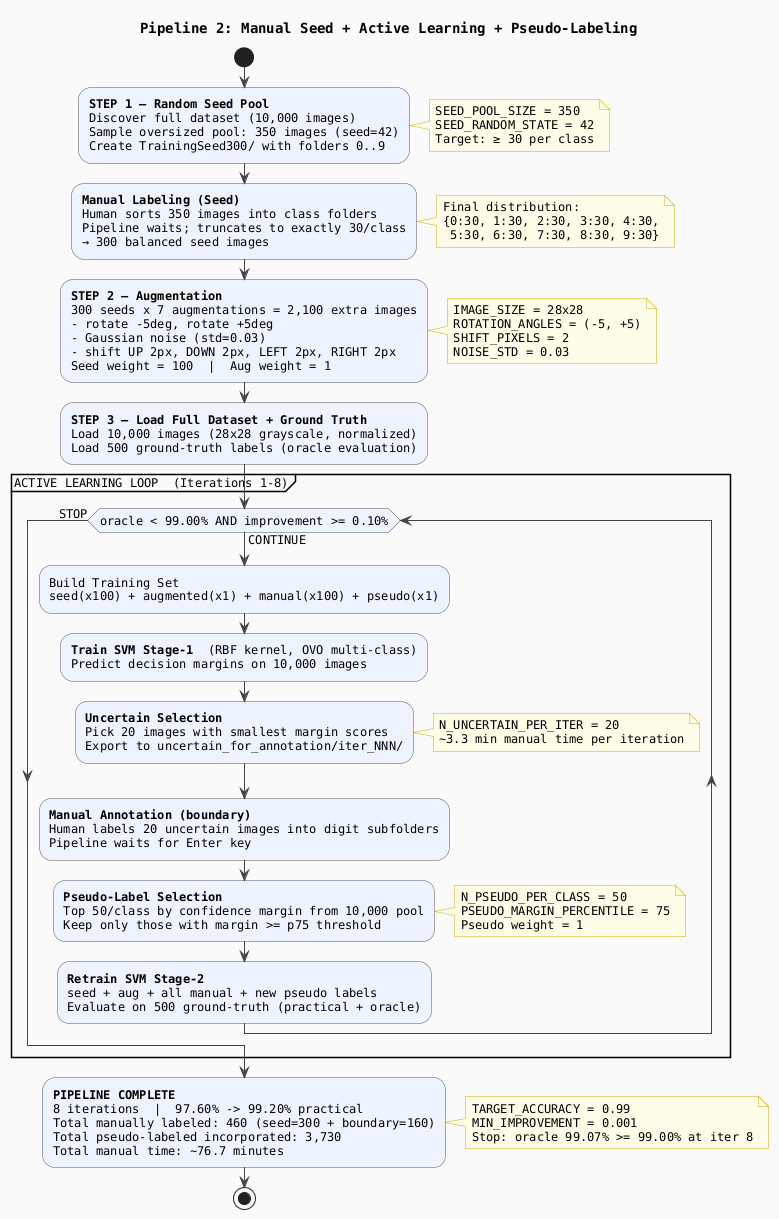
\includegraphics[width=0.6\textwidth]{figures/pipeline2/block diagram.png}
    \caption{Flow chart for pipeline 2 with the exact steps and values}
    \label{fig:pipeline2_block}
\end{figure}
\textbf{Pipeline Workflow}\\
The script follows this iterative lifecycle:
\begin{enumerate}
    \item Load and validate seed data.
    \item Augment seed images (7 synthetic samples per seed image).
    \item Train stage-1 SVM.
    \item Predict on full dataset.
    \item Export 20 most uncertain images for manual labeling.
    \item Wait for manual labels to be completed.
    \item Select high-confidence pseudo-labels from current predictions.
    \item Retrain stage-2 SVM with new manual + pseudo-labeled samples.
    \item Evaluate and check stopping criteria.
    \item If stopping criteria not met, return to step 4 with the retrained model.
\end{enumerate}
\textbf{Stopping Criteria}\\
The loop stops when one of the following is true:
\begin{itemize}
    \item Accuracy is at least 99%.
    \item Iteration-to-iteration improvement is below 0.1%.
\end{itemize}
If oracle evaluation is available, stopping uses oracle accuracy; otherwise practical accuracy is used.

\subsubsection{Simulation results}

\paragraph{Run setup and seed construction.}
The finalized run used all \textbf{10,000} images in \texttt{Indian\_Digits\_Train}. A random oversized pool of 350 images was first sampled for manual organization into class folders, then truncated to a balanced seed set of \textbf{300 images} (30 per class).
Each seed image produced \textbf{7} augmentations (2 rotations, 1 noise variant, and 4 directional shifts), giving \textbf{2100} augmented samples. A fixed practical subset of 500 labeled images was used for in-loop monitoring, and oracle scoring was computed with \texttt{check\_accuracy.p} after each iteration.

\paragraph{Iteration metrics.}
\begin{table}[H]
\centering
\caption{Pipeline 2 iteration metrics (active learning + pseudo-labeling)}
\label{tab:part3_pipeline2_iterations}
\resizebox{\textwidth}{!}{
\begin{tabular}{ccccccc}
\toprule
\textbf{Iter.} & \textbf{Practical (\%)} & \textbf{Oracle (\%)} & \textbf{Manual +} & \textbf{Pseudo +} & \textbf{Rejected (top-50/class)} & \textbf{Threshold} \\
\midrule
1 & 97.60 & 97.64 & 20 & 462 & 38/500 & 0.9933 \\
2 & 98.00 & 97.74 & 20 & 461 & 39/500 & 0.9942 \\
3 & 97.60 & 98.33 & 20 & 454 & 46/500 & 0.9946 \\
4 & 98.20 & 98.51 & 20 & 466 & 34/500 & 0.9948 \\
5 & 98.40 & 98.73 & 20 & 483 & 17/500 & 0.9945 \\
6 & 98.80 & 98.87 & 20 & 473 & 27/500 & 0.9949 \\
7 & 99.00 & 98.97 & 20 & 451 & 49/500 & 0.9953 \\
8 & 99.20 & 99.07 & 20 & 480 & 20/500 & 0.9949 \\
\bottomrule
\end{tabular}
}
\end{table}

\paragraph{Stopping condition and final totals.}
Stopping occurred at iteration 8 when the oracle target was reached:
\[
99.07\% \ge 99.00\%.
\]

\begin{itemize}
    \item Final practical accuracy: \textbf{99.20\%} (496/500).
    \item Final oracle accuracy: \textbf{99.07\%} (9907/10000).
    \item Iterations performed: \textbf{8}.
    \item Total manually labeled images: \textbf{460} (= 300 seed + 160 uncertain samples).
    \item Total pseudo-labeled images incorporated: \textbf{3730}.
    \item Estimated manual time: \textbf{4600 s} ($\approx 76.7$ min), using 10 s per manual label.
\end{itemize}

The active-learning loop improved practical measured accuracy from 97.60\% to 99.20\% and reached the assignment target on oracle evaluation.
